\documentclass[UTF-8,a4paper,zihao=-4]{ctexart}
\usepackage[a4paper,left=3cm,right=2.5cm,top=3cm,bottom=2.5cm]{geometry}
\usepackage{graphicx} % Required for inserting images
\usepackage[backend=biber,style=gb7714-2015]{biblatex} 
\usepackage[labelfont=bf,textfont=bf]{caption}
\addbibresource{ref.bib} %待补上参考文献 
\usepackage{amsmath,amssymb}   % 公式
\usepackage{graphicx}          % 插图
\usepackage{booktabs}           % 三线表
\usepackage{hyperref}           % 超链接（最后加载，少数例外）
\usepackage{placeins}
\usepackage{subcaption}
\usepackage{csvsimple}
\usepackage{listings}
\usepackage{xcolor}
\usepackage{float}
\pagestyle{plain} 
\ctexset{
  section = {
    number = \chinese{section},   % 中文数字：一、二、三…
    format = \zihao{3}\heiti\centering,
    aftername = \quad,            % 编号和标题之间的空格（可调）
    % 如果你想变成“一、绪论”（带顿号），把 aftername 改成 \hspace{1em} 或直接写顿号
  }
}
\makeatletter
\renewcommand{\maketitle}{
    \begin{center}
        \vspace*{-2cm}
        {\zihao{2}\heiti\@title\par}
    \end{center}
}
\makeatother

\makeatletter
\renewenvironment{abstract}
{
    \begin{center}
        {\zihao{-3}\textbf{摘要}}
    \end{center}
    \zihao{-4}
}
{}
\makeatother

\lstset{
    language=Python,
    basicstyle=\ttfamily\small,
    numbers=left,
    numberstyle=\tiny,
    frame=single,
    breaklines=true,
    columns=fullflexible
}

\begin{document}

\title{基于纯方位信息的无人机编队无源定位与队形调整研究}
\date{}
\maketitle

\begin{abstract}

    \textbf{针对问题一(1)：}问题一（1）属于基于方向角信息的二维无源定位问题。本文以 FY00 为原点建立\textbf{平面直角坐标系}描述无人机位置关系，并利用\textbf{圆周角定理}将方向夹角约束转化为\textbf{定角圆约束}。通过构造两组独立角度对应的定角圆，利用\textbf{圆交点}确定接收无人机的位置。

    \textbf{针对问题一(2)：}针对部分发射无人机编号未知的问题，利用圆形编队中无人机均匀分布形成的离散角度特征，建立基于方向夹角匹配的身份识别模型。通过分析不同无人机组合对应的理论夹角范围，实现未知发射无人机编号判定，并结合问题一（1）的定位模型完成偏移无人机的位置确定。结果表明，除已知的 FY00 和 FY01 外，仅需增加一架辅助发射无人机即可实现有效定位。

    \textbf{针对问题一(3)：}

    \textbf{针对问题二：}

\noindent \textbf{关键词：} 
\end{abstract}

\newpage
\section{问题背景与重述}
\subsection{问题背景}

无人机集群执行编队飞行任务时，需要实时掌握各无人机之间的相对位置，以保证队形稳定和飞行安全。然而，在存在外界电磁干扰或隐蔽飞行要求的环境中，若所有无人机频繁主动发射电磁信号，不仅容易受到干扰，还可能暴露集群的位置。因此，无人机集群应尽量保持电磁静默，减少主动信号的发射次数。

纯方位无源定位主要利用接收端获得的方向角信息确定自身位置，不需要测量无人机之间的距离。具体而言，可在编队中选取少量无人机主动发射信号，其余无人机保持被动接收状态，并根据自身与任意两架发射无人机连线之间的夹角，判断当前位置与理想编队位置之间的偏差，进而完成位置调整。这种方法能够在降低通信频率和电磁暴露风险的同时，为无人机编队的队形保持提供有效的位置依据。

在该编队中，每架无人机均具有唯一且固定的编号，其在理想队形中的相对位置关系也保持确定。当多架无人机发射信号时，被动接收信号的无人机可以获得指向不同发射无人机的方向，并进一步提取相邻方向之间的夹角。如图~\ref{fig:direct-diag}，当 FY01、FY02 和 FY03 发射信号时，FY04 可获得三条方向连线之间形成的夹角信息$\alpha_1$、$\alpha_2$和$\alpha_3$。因此，如何利用这些纯方位角信息完成无人机定位，并据此制定合理的队形调整方案，是本文需要解决的主要问题。

\begin{figure}[H]
    \centering
    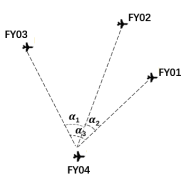
\includegraphics[width=0.4\linewidth]{pic/alpha.png}
    \caption{无人机接收到的方向信息示意图}
    \label{fig:direct-diag}
\end{figure}

\subsection{问题要求}

针对无人机编队飞行中的纯方位无源定位与位置调整问题，需要建立数学模型完成以下四个问题。：
\begin{enumerate}
    \item 对于由 10 架无人机组成的圆形编队，FY00 位于圆心，其余 9 架无人机均匀分布在同一圆周上。现由 FY00 和圆周上的另外两架无人机发射信号，其位置不存在偏差且编号已知，其余位置发生轻微偏移的无人机被动接收信号。要求利用接收到的方向夹角信息，建立被动接收无人机的定位模型，确定其实际位置。
    
    \item 某架位置略有偏差的无人机能够接收到 FY00 和 FY01 发射的信号，同时还能接收到若干架编号未知的圆周无人机所发射的信号。假设所有发射无人机均处于准确位置，分析除 FY00 和 FY01 外，至少还需要安排多少架无人机发射信号，才能消除编号不确定性并实现接收无人机的有效定位。
    
    \item 在理想圆形编队中，FY00 位于圆心，另外 9 架无人机应均匀分布在半径为100m的圆周上。现各无人机初始位置均存在一定偏差，需要设计合理的分步调整方案。每次调整时，可选取 FY00 以及圆周上不超过 3 架无人机发射信号，其余无人机根据接收到的纯方位信息调整位置。在忽略单次调整时间的条件下，使圆周上的 9 架无人机经过多次调整后均匀分布于同一圆周，并结合题目给出的初始位置数据，给出具体的无人机选择顺序和位置调整结果。
    
    \item 将上述纯方位无源定位与调整方法推广至其他无人机编队形式。以直线上相邻无人机间距相等的锥形编队为例，在给定相邻无人机标准间距的条件下，分析其几何结构和位置关系，建立适用于锥形编队的无源定位模型，并设计相应的无人机位置调整方案。
    
\end{enumerate}

\section{问题分析}
\subsection{问题一(1)分析}
问题一（1）需要解决定位问题，我们已知编队中发射信号无人机的位置，而接收无人机仅能够获得自身与发射无人机之间的方向夹角信息，因此该问题本质上属于基于角度约束的二维无源定位问题。由于圆形编队中无人机位置具有明确的极坐标结构，首先本文建立以 FY00 为原点的平面直角坐标系描述各无人机的位置关系。进一步利用圆周角定理，将接收无人机观测到的夹角约束转化为定角圆约束。当仅考虑一组角度信息时，接收无人机的位置只能确定在某一定角圆上，因此需要利用两组独立方向角信息构造两个定角圆，通过两个圆的交点唯一确定无人机的位置。

\subsection{问题一(2)分析}

问题一（2）在问题一（1）的基础上增加了发射无人机编号未知的约束条件。由于圆形编队中无人机均匀分布于同一圆周，因此任意两架圆周无人机之间的圆心角均为 40
∘
 的整数倍，由圆周角定理可知，接收无人机获得的方向夹角具有明显的离散性。利用该性质，可以根据接收到的角度信息判断未知编号发射无人机的位置范围。

具体而言，设偏移无人机为 FY0i，已知发射无人机为 FY00 和 FY01，另选一架编号未知的无人机 FY0j 作为辅助发射机。通过分析 FY00、FY01、FY0j 三者与 FY0i 之间形成的方向夹角，将观测角度分解为理想编队角度与位置偏差项之和，并利用正九边形结构下角度取值规律确定 FY0j 的编号。当未知发射无人机身份确定后，即可利用问题一（1）中的定位模型进一步求解 FY0i 的实际位置。因此，问题一（2）的关键在于利用编队几何约束完成未知发射机身份识别。

\subsection{问题一(3)分析}

\subsection{问题二分析}


%%%%%准备工作%%%%%
\section{初步准备}
\subsection{模型假设}
\begin{enumerate}
    \item 无人机基于自身感知高度信息，保持同一高度，模型由此转为二维平面模型
    \item 无人机位置的偏差是很小的
    \item 
    \item 
    
\end{enumerate}

%%表%%
\subsection{符号说明}
本文所使用的符号及说明如下表所示。
\begin{table}[H]
\centering
\zihao{5}

\caption{符号说明}
\begin{tabular}{ccc}
\toprule
符号 & 说明 & 单位 \\
\midrule
$\rho$ & 极径 & m \\
$\theta$ & 极角 & rad \\
\bottomrule
\end{tabular}

\vspace{0.5em}
\parbox{0.9\textwidth}{
\zihao{5}
注：其他符号已在相应部分中说明。
}
\end{table}

%%%%%模型建立与求解%%%%%
\section{模型建立与求解}
\subsection{问题一(1)的模型建立与求解}
\subsubsection{模型建立}
以FY00为原点，建立平面直角坐标系，则FY00坐标为$O(0,0)$，设圆周半径为R，记第i架无人机为
\begin{equation}
    P_i=(Rcos\theta_i, Rsin\theta_i)
\end{equation}
其中：
\begin{equation}
    \theta_i=(i-1)\frac{2\pi}{9}
\end{equation}
设接收信号的无人机的位置坐标为$(\rho cos\theta,\rho sin \theta)$,

\subsubsection{求解过程与结果}

\subsection{问题一(2)的求解}
\subsubsection{引理与证明}
\begin{enumerate}
\item \textbf{引理}

如图，$A_1A_2...A_9$为正九边形在其外接圆上的九个顶点，其中对于任意三个点形成的圆周角$\alpha$，存在正整数k(k=1,2,3,4,5,6,7)，使得$\alpha=20k^\circ$，对于任意两个点与圆心形成的半径与弦的夹角$\beta$，存在整数l(l=0,1,2,3,4)，使得$\beta=70^\circ-20l^\circ$。
\begin{figure}[H]
    \centering
    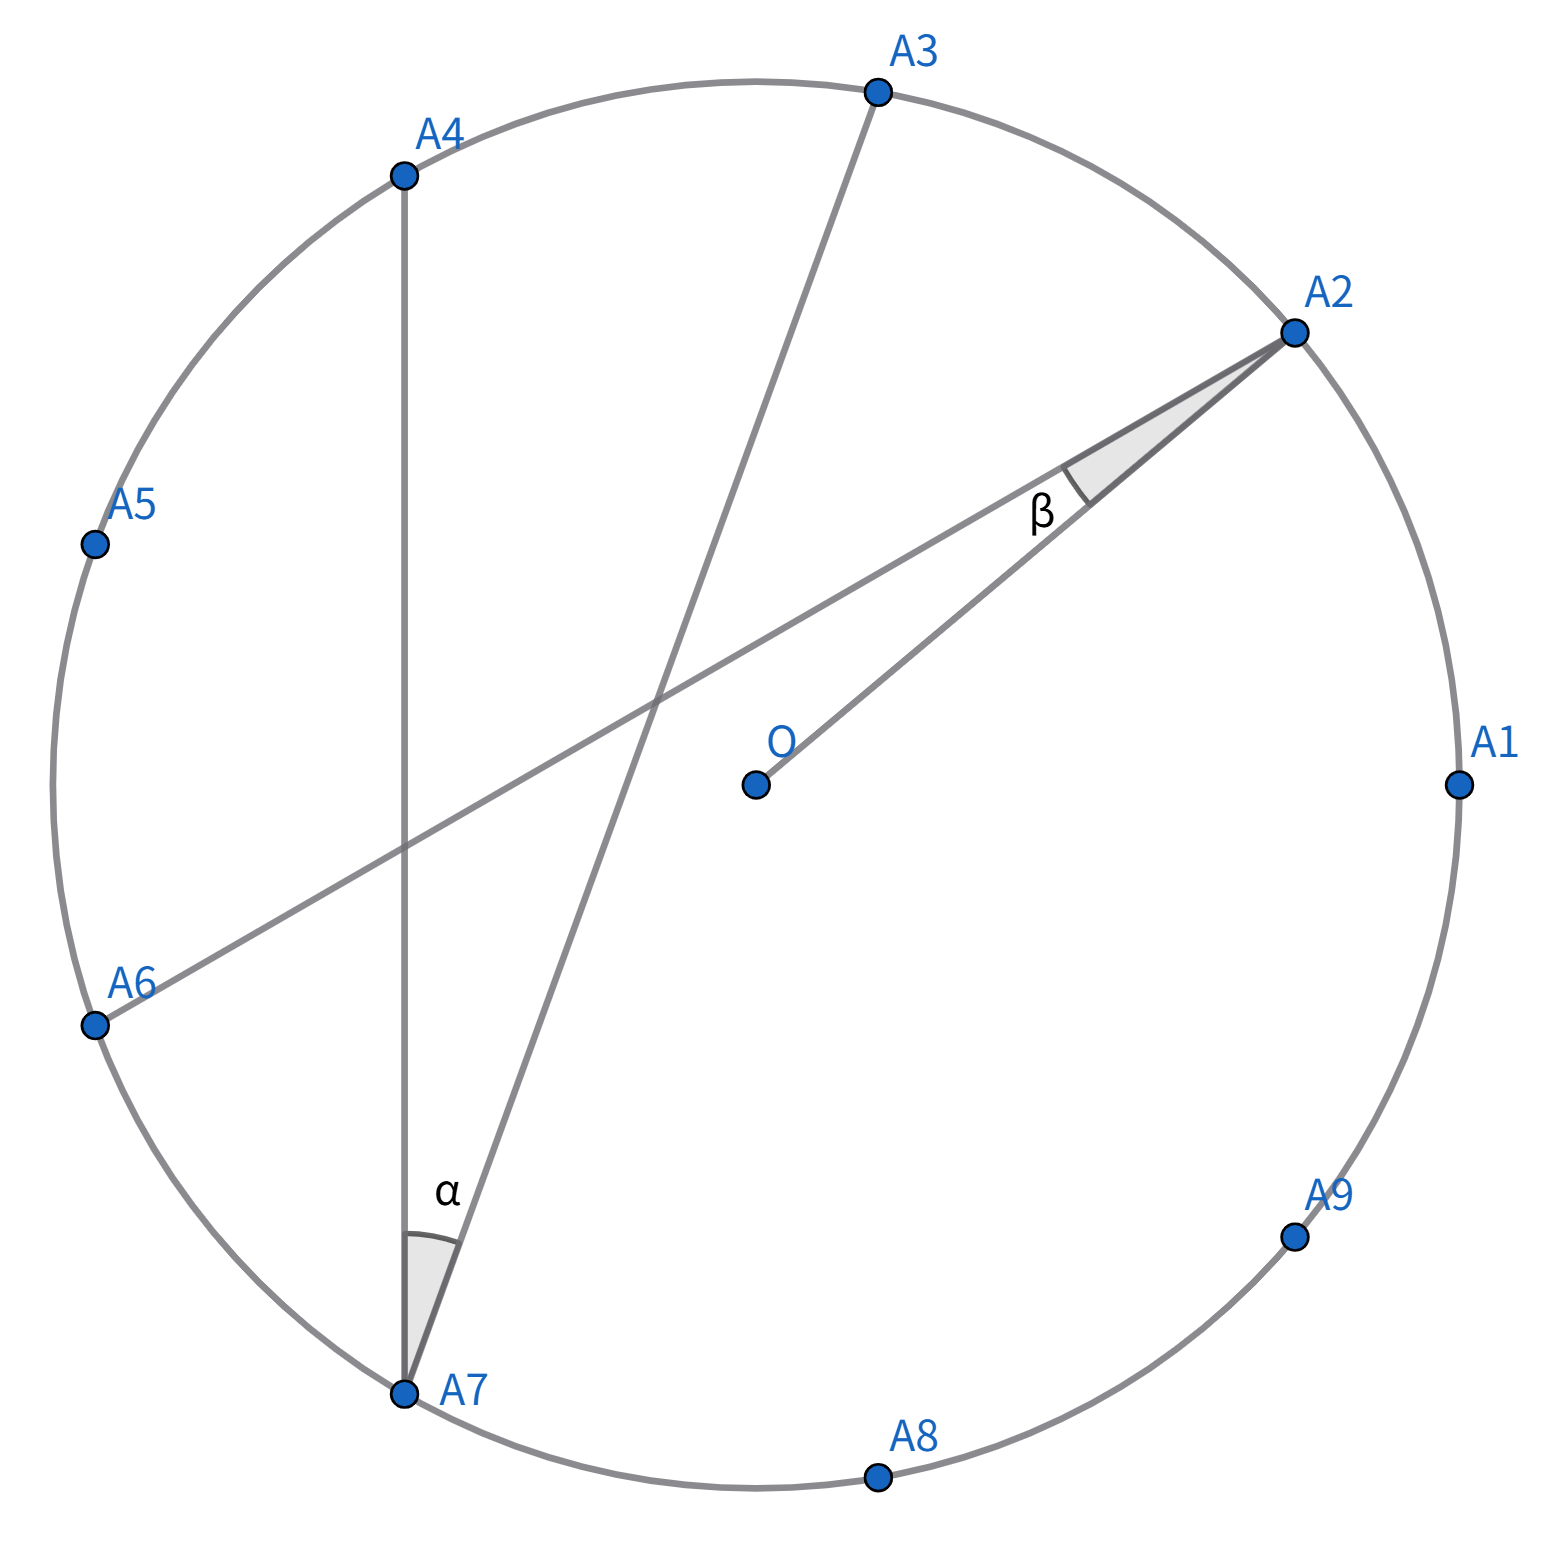
\includegraphics[width=0.8\linewidth]{pic/cir_arc.png}
    \caption{圆周角和半径与弦的夹角示意图}
    \label{fig:direct-diag}
\end{figure}
\item \textbf{证明}

如图，对于一个正九边形，其圆心角一定是$40^\circ$的整数倍，即对于$\angle A_iOA_j(i\neq j)$,存在正整数k(k=1,2,3,4,5,6,7),使得$\angle A_iOA_j=40k^\circ$，所以其对应的圆周角就是$\alpha=20k^\circ$，对于半径与弦的夹角，我们可以知道这个角是以其圆心角为顶角的圆心角的底角，所以存在整数l(l=0,1,2,3,4)，使$\beta=90^\circ-20k^\circ=70^\circ-20l^\circ$。
\begin{figure}[H]
    \centering
    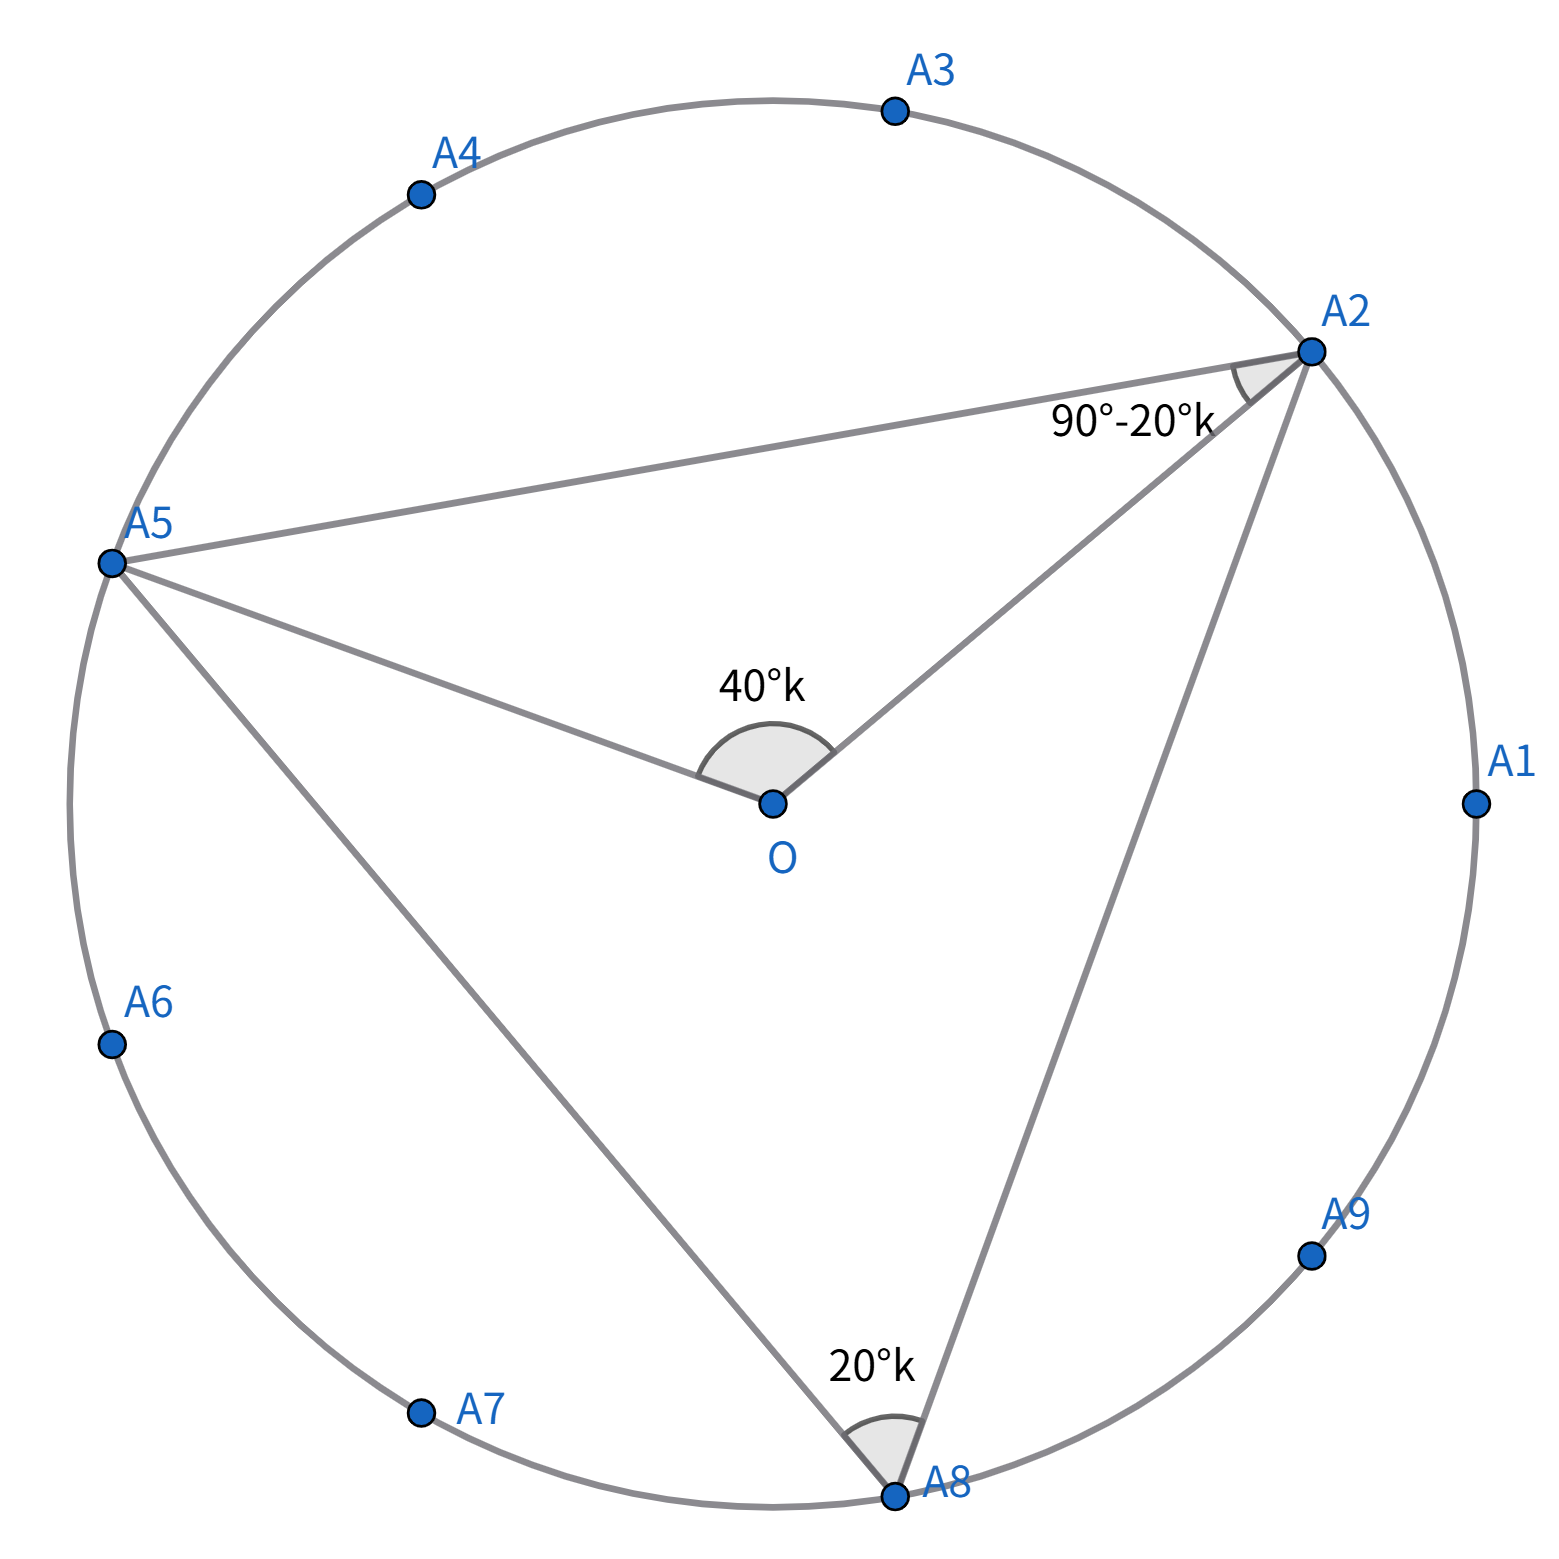
\includegraphics[width=0.8\linewidth]{pic/arc_k.png}
    \caption{圆周角和半径与弦的夹角计算示意图}
    \label{fig:direct-diag}
\end{figure}
\end{enumerate}

\subsubsection{问题求解}
通过引理我们可以知道，对于一个无人机FY0i，其接收到其他无人机的方向信息应该是固定的。所以，对于这个位置略有偏差的无人机，设其为FY0i，我们可以知道它接收到来自FY00和FY01的方向信息为$\angle \theta_{0i1}=70^\circ-{20l_1}^\circ+d_1^\circ$，接收到来自FY00和编号未知但位置无偏差的无人机FY0j的方向信息为$\angle \theta_{0i1}=70^\circ-{20l_j}^\circ+d_2^\circ$,接收到来自FY01和FY0j的方向信息为$20k^\circ+d_3^\circ$,其中$l_1$表示FY01与FY0i之间间隔的顶点数量，其中$l_j$表示FY01与FY0j之间间隔的顶点数量，$d_1^\circ,d_2^\circ,d_3^\circ$表示其偏差值。

所以我们可以根据FY0i收到的三个角度的大致范围，先根据其是10的奇数倍还是偶数倍来判断这些角度分别是来自哪两架无人机的位置信息，再根据FY0i和FY01的关系，将$l_1$和$l_j$区分开来。

由于无人机的位置偏差是很小的，所以误差d不会影响到其大致范围的判断，即\textbf{l和k的取值是唯一的}，根据$l_j$的大小，我们可以初步将FY0j的范围缩小到两个无人机中的一架，即FY0i顺时针方向数第$l_j+1$架无人机和逆时针方向数第$l_j+1$架无人机；再根据$k$的值就可以从前面的两架无人机中确定出\textbf{唯一}的无人机FY0j

确定出来FY0j之后，我们就有了两个位置正确的无人机位置和在圆心的无人机位置了，可以按照第一问的方法来确定位置有偏差的无人机FY0i的位置了。所以除FY00和FY01外，还需要\textbf{1}架无人机发射信号，才能实现无人机的有效定位。

下图是i=4的例子，其中A和B时FY04出现偏差时可能在的位置，其中FY00和FY04与编号未知的无人机连线形成的角度是$50^\circ+d^\circ$，所以我们可以确定出这个编号未知的无人机只可能是FY02或者FY06，此时再看FY01和FY04与编号未知的无人机连线形成的角度，若是$80^\circ+{d_1}^\circ$，则这架发送信号的无人机是FY06，若是$20^\circ+{d_2}^\circ$，则这架发送信号的无人机是FY02。
\begin{figure}[H]
    \centering
    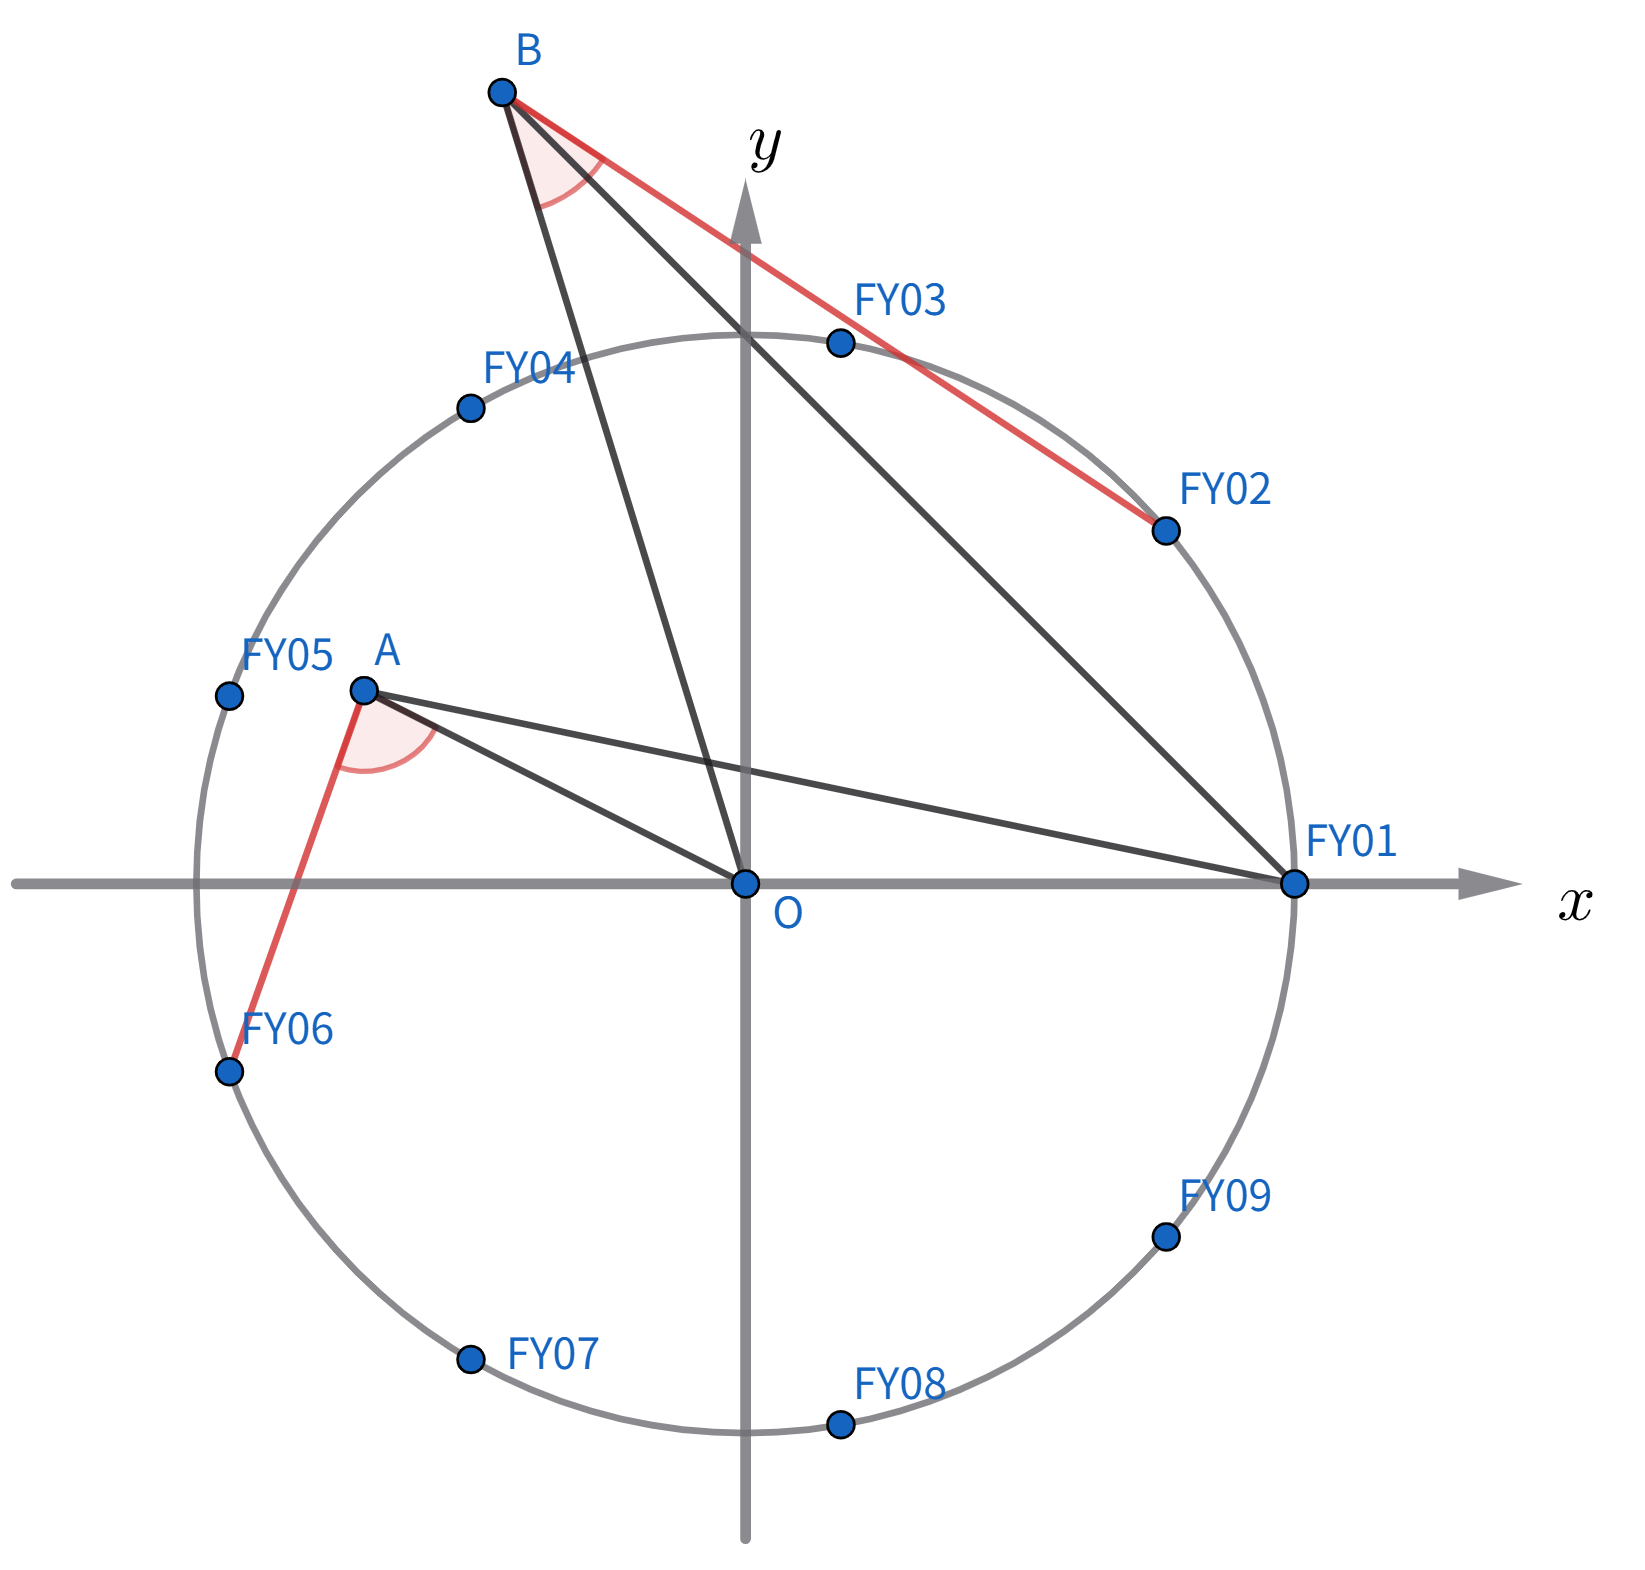
\includegraphics[width=0.8\linewidth]{pic/q1_2.png}
    \caption{问题一(2)例子示意图}
    \label{fig:direct-diag}
\end{figure}
\subsection{问题一(3)的模型建立与求解}
\subsubsection{模型建立}
这一问要求设计一种多轮调整策略，使存在小偏差的圆周无人机逐步回到标准位置。为此，首先需要明确无人机的移动机制。对于任意一架待调整无人机，如果能够确定其当前所在位置，再由其编号确定其理想目标位置，就可以构造一个位移向量，并据此完成位置修正。因此，本问的关键可以归结为两个问题：其一，如何确定接收无人机的当前位置；其二，如何在每一轮中选择发射无人机，使无人机群更快地调整到理想位置。
\vspace{0.5em}
先建立理想编队模板。设圆心无人机 $FY00$ 位于原点，理想圆半径为 $R=100$。第 $i$ 架圆周无人机的理想极角记为 $\theta_i^{*}$，则有
\begin{equation}
\theta_i^{*}=\frac{2\pi(i-1)}{9}, \qquad i=1,2,\dots,9.
\end{equation}
并记第 $t$ 轮时外圈无人机的实际位置为
\begin{equation}
X^{(t)}=\left\{x_1^{(t)},x_2^{(t)},\dots,x_9^{(t)}\right\}.
\end{equation}
由于题目说明各机仅略有偏差，所以可以对其位置进行合理假设
\begin{equation}
x_i^{(t)}=x_i^{*}+\Delta x_i^{(t)}, \qquad \left|\Delta x_i^{(t)}\right|\ll R.
\end{equation}
这一假设说明无人机始终位于对应理想槽位附近，这也是我们后续假定未知无人机坐标的依据。
\vspace{0.5em}
在位置修正层面，设第 $i$ 架无人机在第 $t$ 轮中的当前位置估计为 $\hat{x}_i^{(t)}$，其目标位置为 $x_i^{*}$，那么它的位移向量就可以定义为
\begin{equation}
u_i^{(t)}=x_i^{*}-\hat{x}_i^{(t)}.
\end{equation}
因此，可以建立某一无人机的更新公式为
\begin{equation}
x_i^{(t+1)}=x_i^{(t)}+u_i^{(t)}.
\end{equation}
上式表明：若当前位置估计准确，即满足 $\hat{x}_i^{(t)}=x_i^{(t)}$，则有
\begin{equation}
x_i^{(t+1)}=x_i^{*}.
\end{equation}
这说明在理想情况下，接收无人机可以一步到达理想位置,但是这一理想情况建立在发射无人机的坐标位置均明确的情况下。因此，问题的关键在于如何利用方向信息尽可能准确地估计当前位置，从而加快调整的速度。对于当前位置估计，本文沿用问题一(1)中的纯方位定位思想。设本轮接收机为 $FY0k$，已知准确发射机为 $FY00$ ，再选择若干圆周无人机作为辅助发射机。接收机可观测到由这些发射机构成的夹角信息。若所有发射机位置均已知，则可直接利用两组定角圆求交得到接收机位置。然而在本问中，额外辅助发射机的真实位置本身未知，因此不能直接代入这一精确模型。为解决这个困难，本文从偏差无人机均在理想槽位附近这一假设出发，先通过接收机接收到的角度信息识别发射无人机的编号，再用理想位置对其真实位置进行代换的近似思路进行求解。
设当前接收机为 $FY0r$，候选辅助发射机为 $FY0i$，$FY0j$，$FY0k$中至多三个。在理想编队中，从 $FY0r$ 观察到 $FY0i$ 与 $FY0j$ 的夹角可记为
\begin{equation}
\beta_{i,r,s}^{*}=
\angle\left(x_1^{},x_r^{},x_s^{*}\right).
\end{equation}
对固定的接收机编号 $r$，不同候选发射机编号 $i$ 对应不同的理论特征角。由此可预先构造角度识别特征表，将观测角与理论角进行匹配。设实际观测值为 $\beta_r^{\mathrm{obs}}$，则可按最近邻原则识别辅助发射机编号：
\begin{equation}
\hat{s}=
\arg\min_{s} \left| \beta_r^{\mathrm{obs}}-\beta_{r,s}^{*} \right|.
\end{equation}
当确定发射机编号以后，便可用该发射机的理想位置 $x_{\hat{s}}^{*}$ 替代其真实位置，从而构造近似位移向量。
使用问题一（1）的模型，两组定角圆的非原点交点即为接收机当前位置的一个近似估计点，若本轮选择三架辅助发射机，则可得到两个估计点 。为了降低单个伪锚点近似带来的误差，本文通过取两个估计点的中点来近似接收机的位置。

我们将每次选择发射机后将其他无人机的位置进行一次调整记为一轮调整，为了评价某一轮调整方案的优劣，定义全局损失函数为
\begin{equation}
L=\left(X^{(t)}\right)
\sum_{i=1}^{9} \left| x_i^{(t)}-x_i^{*} \right|_2^2.
\end{equation}
该损失函数统一以位置偏差平方衡量编队状态，即通过描述所有无人机距离理想位置的二范数之和来判断当前无人机群距离理想位置的距离。若记在发射方案 $S_t$ 下执行一轮调整后的状态为 $\mathcal{T}_{S_t}(X^{(t)})$，则单轮最优发射方案满足
\begin{equation}
S_t^{*}=
\arg\min_{S_t} L\left( \mathcal{T}_{S_t}\left(X^{(t)}\right) \right).
\end{equation}
这意味着在每一轮中，都从所有合法的辅助发射机组合中选取使下一轮全局损失最小的方案，即贪心算法。

% % 表格位置说明：此处建议插入“角度识别特征表” \begin{table}[H]
% \centering \caption{角度识别特征表} \label{tab:q1_lookup}
% \begin{tabular}{cccc}
% \toprule 接收机编号 & 候选发射机编号 & 理论角度 & 识别区间 \ \midrule \multicolumn{4}{c}{此处插入表格内容} \ \bottomrule
% \end{tabular}
% \end{table}
\subsubsection{模型的求解}
在上述模型的基础上，本文对问题一第(3)问进行了数值求解。求解过程由``数据预处理--候选方案枚举--单轮贪心更新--收敛判定''四部分组成。
首先进行数据预处理。题目给出的初始位置以极坐标形式表示，设第 $i$ 架无人机的初始极坐标为 $(r_i^{(0)},\theta_i^{(0)})$，则其初始直角坐标为
\begin{equation}
x_i^{(0)}
\begin{bmatrix} r_i^{(0)}\cos\theta_i^{(0)} \ r_i^{(0)}\sin\theta_i^{(0)} \end{bmatrix}, \qquad i=0,1,\dots,9.
\end{equation}
初始无人机位置状态如下
\begin{figure}[H]
\centering \includegraphics[width=0.72\textwidth]{} \caption{初始编队位置示意图} \label{fig:q1_initial}
\end{figure}
与此同时，依据理想模板公式生成全部目标位置 ${x_i^{*}}$，并预先离线生成角度识别特征表。这样在后续每一轮中，只需将接收机观测角与该表进行匹配，即可快速确定未知辅助发射机的编号。
\vspace{0.5em}
其次，枚举每轮全部合法发射机方案。由于 $FY01$ 固定作为参考发射机，因此辅助发射机只需从其余外圈无人机中选取 $1$ 架或 $2$ 架。全部候选集合为
\begin{equation}
\mathcal{S}
\left\{ S\subseteq{FY02,\dots,FY09} \ \middle|
1\le |S|\le 2 \right\}.
\end{equation}
对任意候选方案 $S\in\mathcal{S}$，按如下步骤进行一轮模拟更新：
\begin{enumerate}
\item 固定本轮发射机集合为 ${FY00,FY01}\cup S$； \item 对每架非发射机无人机，根据其观测角识别辅助发射机编号； \item 若本轮选择一架辅助发射机，则由两组定角圆构造一个估计点； \item 若本轮选择两架辅助发射机，则分别构造两个估计点，并取其中点作为当前位置估计； \item 由目标位置与当前位置估计之差构造移动向量，并更新无人机位置； \item 计算该候选方案调整后的全局损失值。
\end{enumerate}
其中，第 $r$ 架接收机在第 $t$ 轮的更新公式为
\begin{equation}
x_r^{(t+1)}=x_r^{(t)}+x_r^{*}-\hat{x}_r^{(t)}.
\end{equation}
因此，若记在方案 $S$ 下的一轮更新结果为 $\mathcal{T}_{S}(X^{(t)})$，则该方案对应的损失为
\begin{equation}
J\left( \mathcal{T}_{S}\left(X^{(t)}\right) \right).
\end{equation}
然后，对所有合法方案逐一比较，选择使损失最小的方案作为本轮最优发射机组合，即
\begin{equation}
S_t^{*}
\arg\min_{S\in\mathcal{S}} J\left( \mathcal{T}_{S}\left(X^{(t)}\right) \right).
\end{equation}
这便构成了单轮贪心算法。由于每一轮都优先选取使下一步误差下降最快的发射方案，因此该策略兼顾了求解效率与实现简洁性。
\vspace{0.5em}
接着给出收敛判据。设收敛阈值为
\begin{equation}
\varepsilon=10^{-4}.
\end{equation}
当满足
\begin{equation}
J\left(X^{(t)}\right)<\varepsilon
\end{equation}
时，认为圆形编队已恢复到题目要求的精度范围内，停止迭代；否则继续执行下一轮贪心调整。由于每一轮都按``最小化下一轮损失''的原则选取发射机方案，因此有
\begin{equation}
J\left(X^{(t+1)}\right)\le J\left(X^{(t)}\right),
\end{equation}
即损失函数保持单调不增。这一性质在程序实现中也得到了逐轮验证。
\vspace{0.5em}
根据代码实现结果，在题目给定初始数据下，该方法共进行 $15$ 轮迭代后达到收敛，最终损失为
\begin{equation}
J\left(X^{(15)}\right)
4.83581741\times 10^{-5} < 10^{-4}.
\end{equation}
这一结果说明，所建立的``角度识别--伪锚点定位--单轮贪心调整''模型能够在发射机数量受限的条件下有效恢复目标编队。需要指出的是，由于辅助发射机的真实位置被其理想位置代替，因此每轮调整并不保证接收机一次精确归位；但随着迭代进行，整体编队越来越接近理想状态，伪锚点近似误差逐步减小，从而保证了模型最终收敛。
此外，若某一轮接收机位置估计完全准确，即有
\begin{equation}
\hat{x}_r^{(t)}=x_r^{(t)},
\end{equation}
则由更新公式立即可得
\begin{equation}
x_r^{(t+1)}=x_r^{*}.
\end{equation}
这表明本文方法在理论上具有明确的几何意义：它本质上是通过不断改进当前位置估计，逐步逼近``一步精确归位''的理想情形。
% % 图片位置说明：此处建议插入“L2损失收敛曲线” \begin{figure}[H]
% \centering \includegraphics[width=0.68\textwidth]{此处替换为图片路径} \caption{$L_2$ 损失收敛曲线} \label{fig:q1_loss}
% \end{figure}
% % 图片位置说明：此处建议插入“多轮调整轨迹图” \begin{figure}[H]
% \centering \includegraphics[width=0.88\textwidth]{此处替换为图片路径} \caption{多轮调整轨迹图} \label{fig:q1_trajectory}
% \end{figure}
% % 图片位置说明：此处建议插入“最终编队位置示意图” \begin{figure}[H]
% \centering \includegraphics[width=0.72\textwidth]{此处替换为图片路径} \caption{最终编队位置示意图} \label{fig:q1_final}
% \end{figure}
% % 表格位置说明：此处建议插入“每轮发射机选择结果表” \begin{table}[H]
% \centering \caption{各轮贪心发射机选择结果} \label{tab:q1_round_choice}
% \begin{tabular}{cccc}
% \toprule 轮次 & 发射机组合 & 调整后损失 & 接收机数量 \ \midrule \multicolumn{4}{c}{此处插入表格内容} \ \bottomrule
% \end{tabular}
% \end{table}
% % 表格位置说明：此处建议插入“最终状态结果表” \begin{table}[H]
% \centering \caption{收敛后无人机极坐标结果} \label{tab:q1_final_state}
% \begin{tabular}{ccc}
% \toprule 无人机编号 & 极径 & 极角 \ \midrule \multicolumn{3}{c}{此处插入表格内容} \ \bottomrule
% \end{tabular}
% \end{table}
综上，问题一第(3)问的求解过程可以概括为：先由题目数据与理想模板建立初始状态；再通过角度识别特征表识别辅助发射机编号；随后对全部合法发射机组合执行单轮贪心搜索，并利用伪锚点近似定位模型完成接收机位置修正；最后在全局损失函数小于阈值时停止迭代并输出结果。该方法满足题目中的发射机数量约束，同时具有清晰的几何解释与稳定的数值收敛性。

\subsection{问题二的模型建立与求解}
\subsubsection{模型建立}

\subsubsection{求解过程与结果}

%%%%%评价%%%%%
\section{模型评价}
\subsection{模型的优点}
\subsubsection{模型具有}

\subsubsection{采用}

\subsection{模型的缺点}
\subsubsection{部分过程}

\subsubsection{未进一步考虑}

%%%%%总结%%%%%
\section{总结}

本文针对

%%%%%参考文献%%%%%
\begin{thebibliography}{99}   % 99 是最大编号宽度

\end{thebibliography}

\section*{附录}
\appendix

\section{文件清单}

\noindent{支撑材料的文件列表清单：}
\begin{enumerate}
    \item result1.xlsx
\end{enumerate}

\section{代码}

\noindent{数据}
\lstinputlisting[language=Python]{}


\noindent{\\ 问题一(1)代码}
\lstinputlisting[language=Python]{}


\noindent{\\ 问题一(2)代码}
\lstinputlisting[language=Python]{}


\noindent{\\ 问题一(3)代码}
\lstinputlisting[language=Python]{}


\noindent{\\ 问题二代码}
\lstinputlisting[language=Python]{}


\end{document}